% ****************************************************************************************
% *********************        SISTEMAS OPERATIVOS            ****************************
% ****************************************************************************************

% =======================================================
% =======         HEADER FOR DOCUMENT        ============
% =======================================================
    % *********   DOCUMENT ITSELF   **************
    \documentclass[12pt, fleqn]{report}                             %Type of docuemtn and size of font and left eq
    \usepackage[margin=1.2in]{geometry}                             %Margins and Geometry pacakge
    \usepackage{ifthen}                                             %Allow simple programming
    \usepackage{hyperref}                                           %Create MetaData for a PDF and LINKS!
    \setlength{\parindent}{0pt}                                     %Eliminate ugly indentation
    \author{Oscar Andrés Rosas}                                     %Who I am

    % *********   LANGUAJE AND UFT-8   *********
    \usepackage[spanish]{babel}                                     %Please use spanish
    \usepackage[utf8]{inputenc}                                     %Please use spanish - UFT
    \usepackage[T1]{fontenc}                                        %Please use spanish
    \usepackage{textcmds}                                           %Allow us to use quoutes
    \usepackage{changepage}                                         %Allow us to use identate paragraphs

    % *********   MATH AND HIS STYLE  *********
    \usepackage{ntheorem, amsmath, amssymb, amsfonts}               %All fucking math, I want all!
    \usepackage{mathrsfs, mathtools, empheq}                        %All fucking math, I want all!
    \usepackage{centernot}                                          %Allow me to negate a symbol
    \decimalpoint                                                   %Use decimal point

    % *********   GRAPHICS AND IMAGES *********
    \usepackage{graphicx}                                           %Allow to create graphics
    \usepackage{wrapfig}                                            %Allow to create images
    \graphicspath{ {Graphics/} }                                    %Where are the images :D

    % *********   LISTS AND TABLES ***********
    \usepackage{listings}                                           %We will be using code here
    \usepackage[inline]{enumitem}                                   %We will need to enumarate
    \usepackage{tasks}                                              %Horizontal lists
    \usepackage{longtable}                                          %Lets make tables awesome
    \usepackage{booktabs}                                           %Lets make tables awesome
    \usepackage{tabularx}                                           %Lets make tables awesome
    \usepackage{multirow}                                           %Lets make tables awesome
    \usepackage{multicol}                                           %Create multicolumns

    % *********   HEADERS AND FOOTERS ********
    \usepackage{fancyhdr}                                           %Lets make awesome headers/footers
    \pagestyle{fancy}                                               %Lets make awesome headers/footers
    \setlength{\headheight}{16pt}                                   %Top line
    \setlength{\parskip}{0.5em}                                     %Top line
    \renewcommand{\footrulewidth}{0.5pt}                            %Bottom line

    \lhead{                                                         %Left Header
        \hyperlink{chapter.\arabic{chapter}}                        %Make a link to the current chapter
        {\normalsize{\textsc{\nouppercase{\leftmark}}}}             %And fot it put the name
    }

    \rhead{                                                         %Right Header
        \hyperlink{section.\arabic{chapter}.\arabic{section}}       %Make a link to the current chapter
            {\footnotesize{\textsc{\nouppercase{\rightmark}}}}      %And fot it put the name
    }

    \rfoot{\textsc{\small{\hyperref[sec:Index]{Ve al Índice}}}}     %This will always be a footer  

    \fancyfoot[L]{                                                  %Algoritm for a changing footer
        \ifthenelse{\isodd{\value{page}}}                           %IF ODD PAGE:
            {\href{https://compilandoconocimiento.com/yo/}          %DO THIS:
                {\footnotesize                                      %Send the page
                    {\textsc{Oscar Andrés Rosas}}}}                 %Send the page
            {\href{https://compilandoconocimiento.com}              %ELSE DO THIS: 
                {\footnotesize                                      %Send the author
                    {\textsc{Compilando Conocimiento}}}}            %Send the author
    }
    
    
    
% ========================================
% ===========   COMMANDS    ==============
% ========================================

    % =====  GENERAL TEXT  ==========
    \newcommand \Quote {\qq}                                        %Use: \Quote to use quotes
    \newcommand \Over {\overline}                                   %Use: \Bar to use just for short
    \newcommand \ForceNewLine {$\Space$\\}                          %Use it in theorems for example
    
    \newenvironment{Indentation}[1][0.75em]                         %Use: \begin{Inde...}[Num]...\end{Inde...}
    {\begin{adjustwidth}{#1}{}}                                     %If you dont put nothing i will use 0.75 em
    {\end{adjustwidth}}                                             %This indentate a paragraph
    \newenvironment{SmallIndentation}[1][0.75em]                    %Use: The same that we upper one, just 
    {\begin{adjustwidth}{#1}{}\begin{footnotesize}}                 %footnotesize size of letter by default
    {\end{footnotesize}\end{adjustwidth}}                           %that's it
        
    % =====  GENERAL MATH  ==========
    \DeclareMathOperator \Space {\quad}                             %Use: \Space for a cool mega space
    \DeclareMathOperator \MiniSpace {\;}                            %Use: \Space for a cool mini space
    \newcommand \Such {\MiniSpace|\MiniSpace}                       %Use: \Such like in sets
    \newcommand \Also {\Space \text{y} \Space}                      %Use: \Also so it's look cool
    \newcommand \Remember[1]{\Space\text{\scriptsize{#1}}}          %Use: \Remember so it's look cool

    \newtheorem{Theorem}{Teorema}[section]                          %Use: \begin{Theorem}[Name]\label{Nombre}...
    \newtheorem{Corollary}{Colorario}[Theorem]                      %Use: \begin{Corollary}[Name]\label{Nombre}...
    \newtheorem{Lemma}[Theorem]{Lemma}                              %Use: \begin{Lemma}[Name]\label{Nombre}...
    \newtheorem{Definition}{Definición}[section]                    %Use: \begin{Definition}[Name]\label{Nombre}...

    \newcommand{\Set}[1]{\left\{ \MiniSpace #1 \MiniSpace \right\}} %Use: \Set {Info}
    \newcommand{\Brackets}[1]{\left[ #1 \right]}                    %Use: \Brackets {Info} 
    \newcommand{\Wrap}[1]{\left( #1 \right)}                        %Use: \Wrap {Info} 
    \newcommand{\pfrac}[2]{\Wrap{\dfrac{#1}{#2}}}                   %Use: Put fractions in parentesis

    \newenvironment{MultiLineEquation}[1]                           %Use: To create MultiLine equations
        {\begin{equation}\begin{alignedat}{#1}}                     %Use: \begin{Multi..}{Num. de Columnas}
        {\end{alignedat}\end{equation}}                             %And.. that's it!
    \newenvironment{MultiLineEquation*}[1]                          %Use: To create MultiLine equations
        {\begin{equation*}\begin{alignedat}{#1}}                    %Use: \begin{Multi..}{Num. de Columnas}
        {\end{alignedat}\end{equation*}}                            %And.. that's it!


    % =====  LOGIC  ==================
    \DeclareMathOperator \doublearrow {\leftrightarrow}             %Use: \doublearrow for a double arrow
    \newcommand \lequal {\MiniSpace \Leftrightarrow \MiniSpace}     %Use: \lequal for a double arrow
    \newcommand \linfire {\MiniSpace \Rightarrow \MiniSpace}        %Use: \lequal for a double arrow
    \newcommand \longto {\longrightarrow}                           %Use: \longto for a long arrow

    % =====  NUMBER THEORY  ==========
    \DeclareMathOperator \Naturals  {\mathbb{N}}                     %Use: \Naturals por Notation
    \DeclareMathOperator \Primes    {\mathbb{P}}                     %Use: \Naturals por Notation
    \DeclareMathOperator \Integers  {\mathbb{Z}}                     %Use: \Integers por Notation
    \DeclareMathOperator \Racionals {\mathbb{Q}}                     %Use: \Racionals por Notation
    \DeclareMathOperator \Reals     {\mathbb{R}}                     %Use: \Reals por Notation
    \DeclareMathOperator \Complexs  {\mathbb{C}}                     %Use: \Complex por Notation

    % === LINEAL ALGEBRA & VECTORS ===
    \DeclareMathOperator \LinealTransformation {\mathcal{T}}        %Use: \LinealTransformation for a cool T

    \newcommand{\pVector}[1]{                                       %Use: \pVector {Matrix Notation} use parentesis
        \ensuremath{\begin{pmatrix}#1\end{pmatrix}}                 %Example: \pVector{a\\b\\c} or \pVector{a&b&c} 
    }
    \newcommand{\lVector}[1]{                                       %Use: \lVector {Matrix Notation} use a abs 
        \ensuremath{\begin{vmatrix}#1\end{vmatrix}}                 %Example: \lVector{a\\b\\c} or \lVector{a&b&c} 
    }
    \newcommand{\bVector}[1]{                                       %Use: \bVector {Matrix Notation} use a brackets 
        \ensuremath{\begin{bmatrix}#1\end{bmatrix}}                 %Example: \bVector{a\\b\\c} or \bVector{a&b&c} 
    }
    \newcommand{\Vector}[1]{                                        %Use: \Vector {Matrix Notation} no parentesis
        \ensuremath{\begin{matrix}#1\end{matrix}}                   %Example: \Vector{a\\b\\c} or \Vector{a&b&c}
    }
    \newcommand{\uvec}[1]{\boldsymbol{\hat{\textbf{$#1$}}}}         %Use: Unitary Vector

    % MATRIX
    \makeatletter                                                   %Example: \begin{matrix}[cc|c]
    \renewcommand*\env@matrix[1][*\c@MaxMatrixCols c] {             %WTF! IS THIS
        \hskip -\arraycolsep                                        %WTF! IS THIS
        \let\@ifnextchar\new@ifnextchar                             %WTF! IS THIS
        \array{#1}                                                  %WTF! IS THIS
    }                                                               %WTF! IS THIS
    \makeatother                                                    %WTF! IS THIS

    % TRIGONOMETRIC FUNCTIONS
    \newcommand{\Cos}[1]{\cos\Wrap{#1}}
    \newcommand{\Sin}[1]{\sin\Wrap{#1}}

    % === CALCULUS ===                               
    \newcommand \Derivate[2] {\dfrac{d #1}{d#2}}                    %Use: Derivate Notation
    \newcommand \Partial[2] {\dfrac{\partial #1}{\partial#2}}       %Use: Derivate Partial Notation
    
    \newcommand \pDerivate[2]{\Derivate{\Wrap{#1}}{#2}}             %But with cool parentesis
    \newcommand \pPartial[2]{\Partial{\Wrap{#1}}{#2}}               %Use: Derivate Partial
    
    \newcommand \SemiDerivate[1]{\Wrap{\dfrac{d}{d#1}}}             %Use: Derivate Notation
    \newcommand \SemiPartial[1]{\Wrap{\dfrac{\partial}{\partial#1}}}%Use: Derivate Partial Notation


    % === COMPLEX ANALYSIS ===
    \newcommand \Cis[1]  {\Cos{#1} + i \Sin{#1}}                    %Use: \Cis for cos(x) + i sin(x)
    \newcommand \pCis[1] {\Wrap{\Cis{#1}}}                          %Use: \pCis for the same ut parantesis



% =====================================================
% ============     	  COVER PAGE	   ================
% =====================================================
\begin{document}
\begin{titlepage}

	\center
	% ============ UNIVERSITY NAME AND DATA =========
	\textbf{\textsc{\Large Proyecto Compilando Conocimiento}}\\[1.0cm] 
	\textsc{\Large Programación}\\[1.0cm] 

	% ============ NAME OF THE DOCUMENT  ============
	\rule{\linewidth}{0.5mm} \\[1.0cm]
		{ \huge \bfseries Bases de Datos}\\[1.0cm] 
	\rule{\linewidth}{0.5mm} \\[2.0cm]
	
	% ====== SEMI TITLE ==========
	{\LARGE Una Pequeña (Gran) Introducción}\\[7cm] 
	
	% ============  MY INFORMATION  =================
	\begin{center} \large
    \textbf{\textsc{Autores:}}\\
        Rosas Hernandez Oscar Andrés \\
        Lopez Manriquez Angel
    \end{center}

	\vfill

\end{titlepage}

% =====================================================
% ========                INDICE              =========
% =====================================================
\tableofcontents{}
\label{sec:Index}

\clearpage




% //////////////////////////////////////////////////////////////////////////////////////////////////////////
% ///////////////////////////////////         SISTEMAS DE COORDENADAS      /////////////////////////////////
% //////////////////////////////////////////////////////////////////////////////////////////////////////////
\part{Parte Abstracta}
\clearpage


    % ===============================================================================
    % ===================           DEFINICIONES               ======================
    % ===============================================================================
    \chapter{Definiciónes}

        % ==============================================
        % ========    REPOSITORIO DE DATOS     =========
        % ==============================================
        \clearpage
        \section{Repositorio de Datos}
            
            Son un conjunto de datos, donde definio a un dato como cualquier información
            que sea váliosa.


        % ==============================================
        % ========        BASE DE DATOS        =========
        % ==============================================
        \clearpage
        \section{Base de Datos}

            Son un conjunto de datos, definido por un modelo de datos, esto no lo tiene necesariamente 
            un repositorio de datos.

            % ==============================================
            % ===    ELEMENTOS DE UNA BASE DE DATOS   ======
            % ==============================================
            \clearpage
            \subsection{Elementos de un Sistema de Base de Datos}

                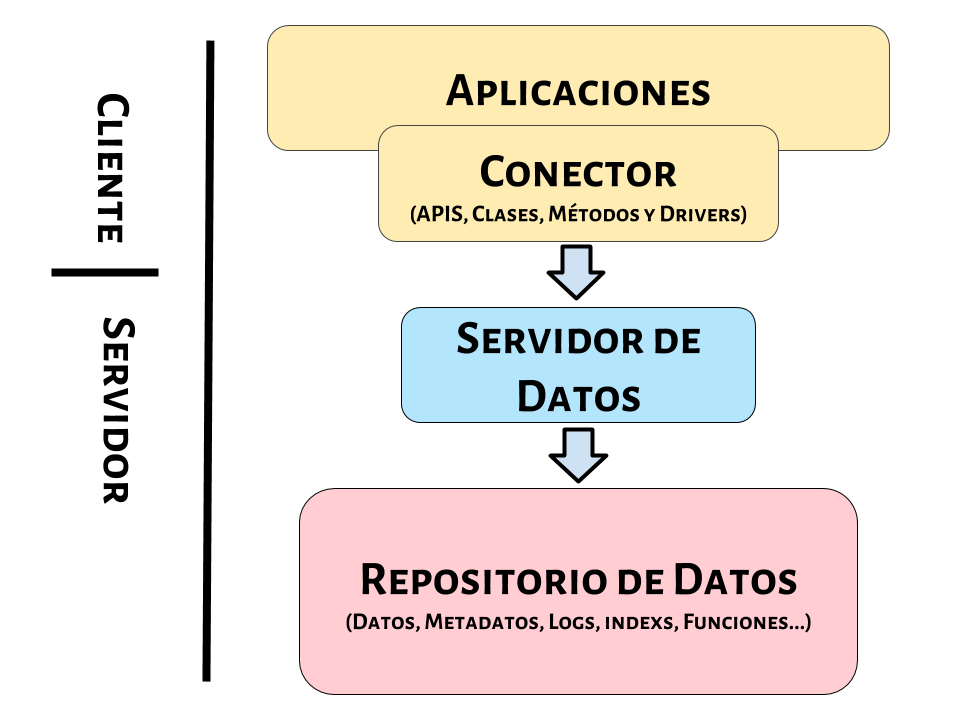
\includegraphics[width=0.85\textwidth]{DiagramaPartes.png}

                \begin{itemize}
                    \item
                        \textbf{Aplicaciones}: Son las aplicaciones que usan la Base de Datos, generalmente creado
                        en lenguajes de Alto Nivel.

                    \item
                        \textbf{Conector:}Son las Apis, o las funciones que permiten a la aplicación interactuar
                        con nuestra base de datos.

                    \item
                        \textbf{Servidor de Datos:}Son el software especialízado qu nos permite manipular
                        inteligentemente nuestro datos:

                        \begin{itemize}
                            \item Creación de Repositorios
                            \item Creación de Cuentas de Usuarios
                            \item Se encarga de crear archivos lógicos, físicos y objetos de la BD.
                            \item Se encarga de administrar las transacciones, bloqueos , etc.
                        \end{itemize}

                \end{itemize}

        % ===============================================
        % ========           METADATOS          =========
        % ===============================================
        \clearpage
        \section{Metadatos}

            Son los archivos que se encargar de definir los esquemas del funcionamiento de la Base de Datos
            sobretodo:
            \begin{itemize}
                \item Nombre y tipo de las tablas
                \item Campos, restricciones y características de cada uno de ellos
            \end{itemize}


        % ===============================================
        % ====     USUARIOS DE UNA BASE DE DATOS     ====
        % ===============================================
        \clearpage
        \section{Usuarios de una Base de Datos}

            \begin{itemize}
                \item
                    \textbf{Administrador de la Base de Datos}

                    Encargado de: 

                        \begin{itemize}
                            \item Monitorear el Performance
                            \item Herramientas Administrativas
                                \begin{itemize}
                                    \item Creacion de cuentas de usuarios
                                    \item Objetos accedidos.
                                    \item Matriz de autorizacion.
                                \end{itemize}
                            \item Definir tiempos de respaldo
                            \item Reorganización físico
                            \item Llevar a cabo las tecnicas de recuperación
                        \end{itemize}

                \item
                    \textbf{Diseñadores de la Base de Datos}

                    \begin{itemize}
                        \item Encargado de grabar los propios Módelos de Datos:
                        
                        \begin{itemize}
                            \item Conceptuales: E/S
                            \item Lógicos: Relacionados
                            \item Físicos: Índices o Estructuras de Datos
                        \end{itemize}

                        \item Esquema de la Base de Datos
                        
                    \end{itemize}


                \item
                    \textbf{Programadores de Aplicaciones}

                    \begin{itemize}
                        \item Interfaces de los usuarios finales
                        \begin{itemize}
                            \item Facilitar el acceso a ciertos "objetos" de la BD
                        \end{itemize}

                        \item Interfaces para la gestión de la aplicaciones 
                        \begin{itemize}
                            \item Operaciones de escritura sobre altas ó bajas 
                            \item IDE desarrollo (Java, .NET)
                            \item Lenguaje Scripts
                            \item Conectividad servidores de datos (API s) 
                        \end{itemize}
        
                    \end{itemize}


            \end{itemize}

            \clearpage
            \subsection{Usuarios Finales}
            \begin{itemize}
                    \item
                        \textbf{Casuales}

                        \begin{itemize}
                            \item Data Minning
                            \item Big Data
                        \end{itemize}

                    \item 
                        \textbf{Principiantes - Paramétricos}
                        :Puntos de venta.

                    \item 
                        \textbf{Sofisticados}
                        \begin{itemize}
                            \item Experiencia en aplicaciones 
                            \item Programadores de aplicación
                            \item DBA 
                            \item Investigadores
                         \end{itemize}
                        
                    \item 
                        \textbf{Independientes (Stand Alone)} 
                            \begin{itemize}
                                \item Sistemas Escolares
                                \item Sistemas de prueba
                                \item Sin conectividad a otros nodos
                            \end{itemize}

            \end{itemize}


        % ===============================================
        % ====    VENTAJAS DE UNA BASE DE DATOS      ====
        % ===============================================
        \clearpage
        \section{Propositos de un Sistema de Base de Datos}

        A diferencias de un Sistema de Archivos, un Sistema de BD
        busca:
        \begin{itemize}
            \item Evitar o miniza la redundancia
            \item Evitar inconsistencias en los datos
            \item Eliminar inconsistencias en los datos
            \item Comunicacion con distintos repositorios de datos
            \item Control de concurrencia
        \end{itemize}




\end{document}










